\section{Introduction}
The world of software engineering has undergone major development and breakthroughs over the past decades, giving birth to numerous workflow models that are used in understanding and examining different types of systems in the business and scientific domains. As defined by Workflow Management Coalition \cite{workflow}, a workflow refers to the automation of a process in which information, documents, or tasks are systematically transferred among participants, following a predetermined set of procedural rules to achieve or contribute to an overall goal. There are three underlying workflow dimensions, namely (1) process, (2) resource, and (3) case, as illustrated in Figure [\ref{workflow_dimensions}]. \par

The \textit{process dimension} is a specification of \textit{processes}, defined as the partial ordering of a set of \textit{tasks} performed by a system \cite{malinao-rdlt}. A \textit{task} is an atomic computation performed by a system, meaning the internal structure of the model is not relevant. The \textit{resource dimension} is a specification of \textit{resources}, such as objects (e.g. user, database, component, etc.) with a determinable set of tasks to perform \cite{malinao-rdlt}. The \textit{case dimension} is a specification of \textit{cases}, which represents an abstract representation of entities or components that are processed from some point of execution of its workflow until its corresponding output is produced \cite{malinao-rdlt}. \textit{Work} is a specification of cases with relevant processes that enable their execution, therefore describing both case and process dimensions. An \textit{activity} is the actual performance of a resource with respect to a work specification, hence profiling all three workflows together \cite{malinao-rdlt}.

\begin{figure}[h]
    \centering
    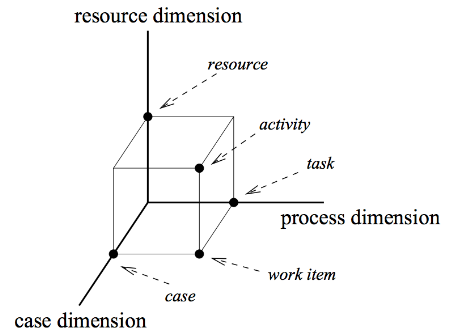
\includegraphics{figures/workflow-dimensions.png}
    \caption{The three dimensions of a workflow \cite{vanderaalst}}
    \label{workflow_dimensions}
\end{figure} \par

Major advancements have led to the introduction and formulation of various workflow models that are capable of representing any or all of the workflow dimensions. Examples under the Unified Modelling Language (UML) are \textit{Class Diagrams} and \textit{Component Diagrams} which are used to represent the resource dimension of a system \cite{uml}. A \textit{Petri net (PN)} provides a graphical notation showing step-by-step computations that are performed when conditions are satisfied given some initial input configuration in the net. PNs are considered multidimensional workflow diagram because it is capable of representing two or more workflow dimensions, i.e. process and case dimensions \cite{yiu}. Another example of a multidimensional workflow model is the Robustness Diagram with Loop and Time Controls (RDLT), which is an extension of the Robustness Diagram, that can capture all three (3) workflow dimensions: process, resource, and case, making it a powerful tool for representing simple and complex systems. The concept of \textit{reset-bound subsystems (RBS)} was formulated and introduced in the RDLT, allowing the simulation of cancellation regions in other well-known workflow diagrams. The subprocess RBS is induced by the $M$-attribute value of a vertex within itself, which is referred to as the \textit{center} of the RBS. The RDLT also offers the capability of restricting the number of traversals along an arc through the use of an $L$-attribute. Real-world applications of RDLTs include profiling the efficiency of the Philippine Integrated Disease Surveillance and Response (PIDSR) system \cite{lopez-etal}, and modeling of the Adsorption Chiller system into RDLT \cite{malinao-rdlt}, among other things. \par

Unlike other models such as Class Diagrams and Petri nets, no automated tool supports the implementation, verification, simulation, and model-to-model decomposition of RDLT. This prompted the exploration of Yiu et al. \cite{yiu} on the partial mapping of RDLT to Class Diagrams and Petri nets, which capture a single dimension (resource), and two out of three dimensions (process and case), respectively. The mapping from RDLT to PN, however, does not include the $L$ and $M$-attributes of the RDLT resulting in a PN that does not support resets and traversal limits on an arc. Drawing inspiration from this gap, Sulla and Malinao \cite{sulla-malinao} formulated a novel mapping for the $L$ and $M$-attributes of RDLT to PN in order to achieve complete mapping of the components. Additionally, their paper reported on the implications of $L$ and $M$-attribute mapping to the soundness of Petri nets. Unfortunately, as a limitation, this proposed mapping was not able to fully capture the functionality of resets and replenishments in RBS. Meaning, tokens are not replenished once exiting the RBS, and reuse is not allowed, unlike RBS in RDLT. \par

To contribute to the development of RDLT analysis, this paper aims to formulate a mapping algorithm of RDLT to PN with considerations of the full functionality of reset-bound subsystems (RBS) and to evaluate if such mapping results in an output PN that is classical or relaxed sound.
    
    \subsection{Background of the Study}
        \subsubsection{Basic Notations and Definitions}
        % \addcontentsline{toc}{subsection}{Robustness Diagram with Loop and Time Controls}
        \subsection*{Robustness Diagram with Loop and Time Controls}
        The \textit{Robustness Diagram with Loop and Time Controls (RDLT)} is an extension of the Robustness Diagram (RD) that captures all three workflow dimensions. It is formally defined in Definition 1.

        \newtheorem{definition}{Definition}

        \begin{definition} \textbf{RDLT} \cite{malinao-rdlt}
        
        An RDLT is a graph representation $R$ of a system that is defined as $R = (V, E, T, M)$ where:

            \begin{itemize}
            
                \item $V$ is a finite set of vertices, where each vertex has a type $V_{type}: V \rightarrow \{'b', 'e', 'c'\}$ where 'b', 'e', and 'c' means the vertex is either a "boundary object", an "entity object", or a "controller", respectively.
                
                \item A finite set of arcs $E \subseteq (V \times V) \backslash  E'$ where $E' = \{(x,y) | x,y \in V, V_{type}(x) \in \{'b', 'e'\}$, $V_{type}(y) \in \{'b', 'e'\}$ with the following attributes with user-defined values,
                
                \begin{itemize}
                    
                    \item $C : E \rightarrow \Sigma \cup \{\epsilon\}$ where $\Sigma$ is a finite non-empty set of symbols and $\epsilon$ is the empty string. Note that for real-world systems, a task $v \in V$, i.e. $V_{type}(v) = $'c', is executed by a component $u \in V, V_{type}(u) \in $ \{'b','e'\}. This component-task association is represented by the arc $(u, v) \in E$ where $C((u,v)) = \epsilon$. Furthermore, $C((x,y)) \in \Sigma$ represents a constraint to be satisfied to reach $y$ from $x$. This constraint can represent either an input requirement or a parameter $C((x,y))$ which needs to be satisfied to proceed from using the component/task $x$ to $y$. $C((x,y)) = \epsilon$ represents a constraint-free process flow to reach $y$ from $x$ or a self-loop when $x = y$.
                    
                    \item $L : E \rightarrow \mathbb{Z}$ is the maximum number of traversals allowed on the arc.
                    
                \end{itemize}
            
                \item Let $T$ be a mapping such that $T((x, y)) = (t1,...,tn)$ for every $(x, y) \in E$ where $n = L((x, y))$ and $ t_{i} \in \mathbb{N}$ is the time a check or traversal is done on $(x, y)$ by some algorithm’s walk on $R$.
                    
                \item $M : V \rightarrow \{0,1\}$ indicates whether $u \in V$ and every $v \in V$ where $(u,v) \in E$ and $C((u,v)) = \epsilon$ induce a sub-graph $G_{u}$ of $R$ known as a \textbf{reset-bound subsystem} (RBS). The RBS $G_{u}$ is induced with the said vertices when $M(u) = 1$. In this case, $u$ is referred to as the \textbf{center} of the RBS $G_{u}$. $G_{u}$'s vertex set $V_{G_{u}}$ contains $u$ and every such $v$, and its arc set $E_{G_{u}}$ has $(x,y) \in E$ if $x,y \in V_{G_{u}}$. \\
                
                Finally, $(a,b) \in E$ is called an \textbf{in-bridge} of $b$ if $a \notin V_{G_{u}}, b \in V_{G_{u}}$. Meanwhile, $(b,a) \in E$ is called an \textbf{out-bridge} of $b$ if $b \in V_{G_{u}}$ and $a \notin V_{G_{u}}$. Arcs $(a,b), (c,d) \in E$ are \textbf{type-alike} if $\exists y \in V$ where $(a,b), (c,d) \in Bridges(y)$ with $Bridges(y) = \{(r,s) \in E|(r,s)$ is either an in-bridge or out-bridge of $y\}$ or if $\forall y \in V, (a,b), (c,d) \notin Bridges(y)$.
                
            \end{itemize}
            
        \end{definition}

        \begin{figure}[h]
            \centering
            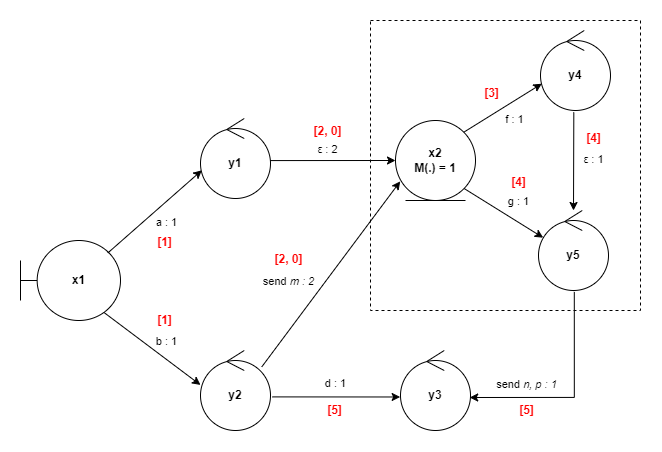
\includegraphics[scale=0.65]{figures/RDLT1.png}
            \caption{An RDLT with 5 controllers, 1 boundary object, 1 entity object, and $T$-attributes in red text. The center of the reset-bound subsystem (RBS) is the vertex x2, with owned controllers y4 and y5 \cite{yiu}.}
            \label{rdlt1}
        \end{figure} \par

        \begin{figure}[h]
            \centering
            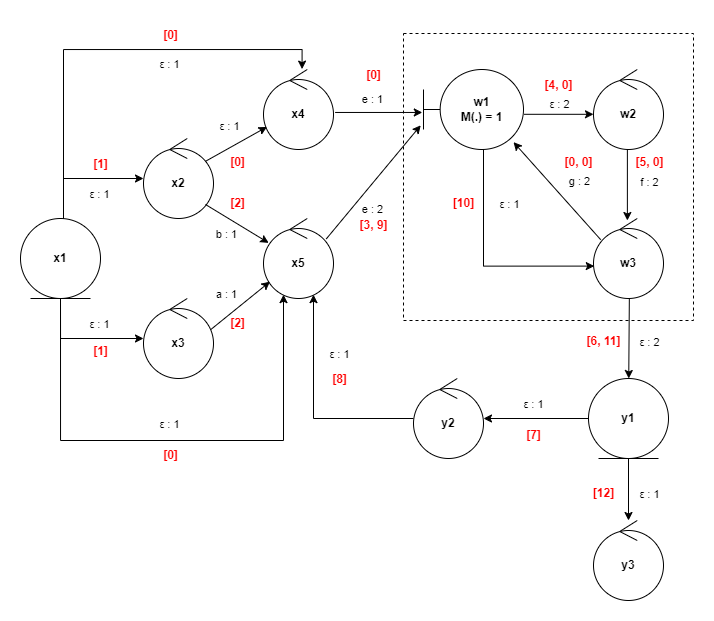
\includegraphics[scale=0.65]{figures/RDLT2_PJS.png}
            \caption{An RDLT with 8 controllers, 1 boundary object, 2 entity objects, and $T$-attributes represented in red text. The center of the reset-bound subsystem (RBS) is the vertex w1, owning controllers w2, and w3 \cite{malinao-pjs}.}
            \label{rdlt2}
        \end{figure} \par

        \begin{definition} \textbf{Vertex Ownership} \cite{yiu}
            
            In an RDLT $R$, a vertex $x \in V$ where $V_{type}(x) \in \{'e','b'\}$ is the \textbf{owner} of a vertex $y \in V$ where $V_{type}(y) = \{'c'\}$ if arc $ (x,y) \in E $ where $ C((x,y)) = \epsilon $. Each $y$ only has one (1) \textbf{owner vertex}. We denote this relationship by $y_{owner} = x $. Arc $ (x,y) $ is an \textbf{ownership arc}.
        
        \end{definition}

        \begin{definition} \textbf{Psuedocritical Arcs, Pseudo-escape Arcs} \cite{malinao-wctp}
            
            A \textbf{pseudocritical arc}(PCA) $(x,y)\in E$, where $(x,y)$ is a component of a cycle $c$ in $R$, where $L(x,y)$ is the minimum among all the $L$-values of the arcs in $c$ which are not arcs of an RBS in $R$.
            Meanwhile, a \textbf{pseudo-escape arc}(PEA) $(x,z) \in E$ is a non-critical arc in $R$ where $(x,y)$ and $(x,z)$ are type-alike.
        
        \end{definition}

        \begin{definition} \textbf{Expanded Reusability in RDLTs with Resets} \label{expanded} \cite{malinao-wctp}

            Let $R=(V,E,T,M)$ be a connected RDLT. If $\exists v \in V$ where $M(v)=1$, then let $B=(V',E',T',M')$ be the RBS with its center $v$.

            Let $IBr(x)$ be the set of in-bridges of $x \in V$

            Let $Cycles_{part}(R)$ be a set of cycles in $R$ where $\forall p=[x_{1}x_{2}...x_{n}]\in Cycles_{part}(R)$, there is at least one cycle component $(x_{i},x_{i+1}) \in E$ that is inside an RBS $B$ of $R$, i.e. $x_{i},x_{i+1} \in V'$, and at least one cycle component $(x_{j},x_{j+i}) \in E$ that is not inside $B$, i.e. $x_{j}$ or $x_{j+1}$ is not in $V'$. Whenever we have cycles $d=[d_{1}d_{2}...d_{m_{1}}]$, $e=[e_{1}e_{2}...e_{m_{2}}] \in Cycles_{part}(R)$ that overlap in their non-RBS components such that this overlap contains both of their $PCAs(d_{k},d_{k+1})$, $(e_{k'},e_{k'+1})$, where $L(d_{k},d_{k+1}) \geq (e_{k'},e_{k'+1})$, we only consider one of these $PCAs$, whichever has the minimum $L$-value since it would ultimately contribute to the reusability of every RBS component that has a path from these cycle components.

            By Definition \ref{expanded}, the expanded reusability $eRU(x,y)$ of the NCA arcs of $R$ with no RBS is equal to $RU(x,y)$ as in literature. Meanwhile, if $(x,y)$ is inside an RBS, its expanded reusability provides the maximum number of times $(x,y)$ can be used by an activity profile in $R$. This $eRU(x,y)$ is determined by the number of times each cycle containing $(x,y)$ is accessed through each of the in-bridges of its components, as well as the number of times it is (re)used inside its RBS. If and when this in-bridge is also part of this cycle, $eRU(x,)$ uses the $L$-value of the PCA of this cycle since this PCA controls the (re)use of $(u,v)$, $(x,y)$, and the cycle itself. On the other hand, if this in-bridge $(u,v)$ is snot part of any cycle that involves $(x,y)$, yet there is a path from $(u,v)$ to $(x,y)$, then $(x,y)$ is used one time in this activity through the traversal of $(u,v)$.
            
        \end{definition}

        \begin{definition} \textbf{RU-preserving transformation} \cite{malinao-wctp}

            A transformation $\delta$ of an input RDLT $R$ to another RDLT $R'$ is said to be \textbf{RU-preserving} if for every activity profile $S=\{S(1),S(2),...,S(n_{1})\}, n_{1} \in \mathbb{N}$, that is derivable from $R$, there is a corresponding activity profile $S'=\{S'(1),S'(2),...,S'(n_{2})\},n_{2} \in \mathbb{N}$, that is derivable from $R'$, where for every pair $(x,y) \in S(i)$ and $(y,z) \in S(i+1)$, either of the following holds:

            \begin{enumerate}
                \item $(x,y) \in S'(j)$ and $(y,z) \in S'(j+1)$,
                \item there exists a path $p=x_{1}x_{2},...,x_{n}$ in $R$ being represented by the arc $(x_{1},x_{n}$ in $R'$ where $x_{k-1}=x,x_{k},=y,x_{k+1},$ and
                    \begin{itemize}
                        \item $(s,x_{1}) \in S'(j)$ and $x_{1},x_{n} \in S'(j+1)$, for some vertices $s$ in $R'$, or
                        \item $(x_{1},x_{n}) \in S'(j)$, or for some $1\leq j \leq n_{2}$, or
                        \item $(x_{1}, x_{n}) \in S'(j)$ and $(x_{n},s) \in S'(j+1)$, for some vertex $s$ in $R'$.
                    \end{itemize}
            \end{enumerate}
                Furthermore, we call $(x_{1},x_{n})$ as the \textbf{abstract arc} in $R'$ representing the path in $R$.
        \end{definition}

        \begin{definition} \textbf{Vertex-simplified RDLT} \cite{malinao-rdlt}

            A vertex-simplified RDLT $G = (V',E',C')$ of $ R = (V,E,\Sigma,C,L,M)$ is a multidigraph whose vertices $v \in V$ have $V_{type}(v) = c$ where $G$ is derived from $R$ such that the following holds:

            \begin{enumerate}
                
                \item $x \in V'$ if any of the following holds:
                    \begin{itemize}
                        
                        \item $x \in V$ and $x \notin {V_G}_u$ of an RBS $G_u$ in $R$, or

                        \item there exists an in-bridge $(q,x) \in E$ of $x \in V \cap {V_G}_u$, $q \in V$ of $R$, or

                        \item there exists an out-bridge $(x,q) \in E$ of $x \in V \cap {V_G}_u$, $q \in V$ of R
                        
                    \end{itemize}

                \item $(x,y) \in E'$ with $C'((x,y)) = C((x,y))$ for $x,y \in V'$ if $(x,y,) \in E$

                \item $C((x,y)) = \epsilon$ if $x,y \in V' \cap {V_G}_u$ and $x$ is an ancestor of $y$ in $R$, $(x,y) \notin {E_G}_u$.
                
            \end{enumerate}
        
        \end{definition}

        The vertex-simplification process abstracts the reset-bound subystems (RBS) and converts each of the vertices present in an RDLT into controllers. This simplification of the $RDLT R$ is referred to as \textbf{level-1 vertex-simplification} of $R$ with respect to every $RBS$ $G_{u}$ in $R$. The \textbf{level-2 vertex-simplification} of $R$ with respect to its $RBS$ $G_{u}$ is the level-1 vertex-simplification of $G_{u}$ where $G_{u}$ is treated as an $RDLT$ where the value of the $M$-attribute of $u$ is set to $0$, i.e. $M(u) = 0$.

        The method presented in  \cite{sulla-malinao} uses vertex simplification to generate the level-1 and level-2 vertex-simplified RDLT as one of its pre-processing steps for its input RDLT. These two RDLTs show the information of the overall RDLT and the information inside the RBS, respectively. The equivalent Petri Nets of these two RDLTs are combined to produce a single Petri Net via XOR split which is then used for model verification.

        % Definition of Expanded vertex simplification here
        \begin{definition} \textbf{Extended Vertex Simplification Algorithm (EVSA)} \cite{malinao-wctp}

            Since the vertex simplification of $R$ used in the literature lacks the $L$-values of its $R_{1}$ and $R_{2}$, this process is extended to produce the \textbf{expanded vertex simplification} $R'_{1}$ and $R'_{2}$ of $R$ by using $R_{1}$, $R_{2}$, and $R$ itself. The expanded version $R'_{1}$ and $R'_{2}$ inherit the vertex and arc sets and attributes of $R_{1}$ and $R_{2}$, respectively, while now having either the original or derived $L$-values of $R$.

            \textbf{Inputs:} Let $R=(V,E,T,M)$ be a connected RDLT with an RBS, i.e. $\exists v \in V$, where $M(v)=1$. Let $R_{1}=(V_{1},E_{1})$ and $R_{2}=(V_{2},E_{2})$ be the vertex simplifications of $R$.
            \textbf{Outputs: Level 1 and Level 2 expanded vertex simplification} $R'_{1}=(V'_{1},E'_{1},T'_{1})$ and $R'_{2}=(V'_{2},E'_{2},T'_{2})$ of $R$, respectively.

            \begin{enumerate}
                \item For each $v \in V_{1}(V_{2})$(or $V$ of $R$), set $v' \in V'_{1}(V'_{2})$ to be its corresponding vertex, and if $(u,v) \in E_{1}(E_{2})$, then there is a corresponding arc $(u',v') \in E'_{1}(E'_{2})$, where the C-values $C'_{1}(u',v')(C_{2}(u',v'))$ of $R'_{1}(R'_2)$ is set to $C(u,v)$ of $R_{1}(R_{2})$, otherwise, none.

                \item For each $(u,v) \in E$, where $(u,v)$ is not in an RBS of $R$, and its corresponding arc $(u',v') \in V'_{1}$ of $L_{1}$, let $L'_{1}(u',v')=L(u,v)$.

                \item For each abstract arc $(u',v') \in E'_{1}$ of $R_{1}$, where $(u',v')$ represents the path $p=x_{1}x_{2}...x_{n}$ in $R$, i.e. $x_{1} \in V$ and $x_{n} \in V$ correspond to $u' \in E'_{1}$ and $v' \in E'_{1}$, respectively, set $L'_{1}(u',v')=min_{i=1,...,n-1} \{eRU(x_{i},x_{i+1})\}+1$.
                
            \end{enumerate}
        
        \end{definition}

        \begin{definition} \textbf{Extended RDLT} \cite{malinao-rdlt}

            An extended RDLT $R' = (V',E',\Sigma,C',L',M)$ is derived from R such that

            \begin{enumerate}
                
                \item $V' = V \cup \{i\} \cup \{o\}$, where i and o are dummy source and sink where $V_{type}(o) = 'c'$.

                \item $E' = E \cup \{(i,u)\} \cup \{(x,o)\}, \forall u \in I\backslash \{i\}, I \subset V, I = \{u \in V | u$ is a source in V $\}, C'((i,x)) = $ '$\epsilon$', $L'((i,x)) = 1$, and $\forall x \in O\backslash \{o\}$, $O \subset V$, $O = \{x \in V | x$ is a sink in $V\}$, $C'((x,o)) = $ '$x\textunderscore \textunderscore o$', $\Sigma := \Sigma \cup \{x\textunderscore\textunderscore o\}$, and $L'((x,o)) = 1$. Note that the new labels are distinguishable from each other.
                
            \end{enumerate}
            
        \end{definition}

        An extended RDLT includes two additional vertices, the source, and the sink, denoted as $i$ and $o$. These vertices are connected to the source and sink vertices of the RDLT, respectively.

        \subsubsection*{Activity Extraction in RDLT}
        
        \begin{definition} \textbf{Unconstrained Arc} \cite{malinao-rdlt}

        Let $R = (V,E,T,M)$ be an RDLT (with the arc attributes C and L). An arc $(x,y) \in E$ is \textbf{unconstrained} if $\forall (v,y) \in E$ where $(x,y)$ and $(v,y)$ are type-alike, any of the following holds,

            \begin{enumerate}
                
                \item $C((v,y)) \in \{\epsilon,C((x,y))\}$,

                \item $|\{t_{i} \in T((x,y))|t_{i} \geq 1\}|\leq |\{t_{j} \in T((v,y))|t_{j} \geq 1\}| \leq L((v,y))$,

                \item $C((v,y)) \in \Sigma \wedge C((x,y)) = \epsilon \wedge T(v,y) \neq 0$.
                
            \end{enumerate}
            
        \end{definition}

        \begin{definition} \textbf{Reachability Configuration} \cite{malinao-rdlt}

        A reachability configuration $S(t)$ in $R$ contains the arcs traversed at time step $t \in \mathbb{N}$.
            
        \end{definition}

        \begin{definition} \textbf{Activity Profile} \cite{malinao-rdlt}

        We call a set $S = S(1), S(2), \ldots, S(d)$ of reachability configurations, $d \in \mathbb{N}$, as an activity profile in $R$ where $\exists(u,v) \in S(1)$ and $(x,y) \in S(d)$ such that $ \nexists w,z \in V$ where $(w,u),(y,z) \in E$.
            
        \end{definition}

        \textbf{Algorithm A}: Activity Extraction \cite{malinao-rdlt}
        \begin{enumerate}
            \item Initialize $S$
            \item For every $(x,y) \in E$, initialize $T((x,y))$ such that $T((x,y)) = (t_{1},\ldots,t_{n})$ where $n = L((x,y))$ and $t_{i} \in \mathbb{N}$ is the time a check/traversal is done on $(x,y)$ by $A$.
            \item Let $x = s$.
            \item While $x \neq f$ do:
                \begin{enumerate}
                    \item Select $(x,y) \in E$ where $L((x,y))$ has not been reached.
                    \item Assign $maxV + 1$ to the leftmost zero of $T((x,y))$. If $\exists(u,x) \in E = max(T((u,x)))$. Otherwise, $maxV = 0$.
                    \item Determine whether $(x,y)$ is an unconstrained arc or not.
                    \item If $(x,y)$ is unconstrained, traverse $(x,y)$ and assign $MAX+1$ to $T((x,y))$. $MAX$ is the maximum value from all $T((v',y)) \forall v' \in V$ where $(v',y),(v,y)$, and $(x,y)$ are type-alike. For every $(v,y) \in E$ that is type-alike with $(x,y)$, assign $MAX+1$ to every $T((x,y))$. If $C((v,y)) \in \Sigma$, the last value in $T((x,y))$ where the last check was done on $(v,y)$ is updated. If either type '$b$' or '$e$' and $y$ is type '$c$', the first value in $T((x,y))$ is updated.
                    \item If $(x,y)$ is not unconstrained and no other $(x,y') \in E$ where $y' \in V$ can be selected, backtrack to $a \in V$ where $(a,x) \in E$ and $a$ was previously visited by A to reach $x$.
                \end{enumerate}
            \item If activity extraction fails, return $\emptyset$. Otherwise, return $S$.
        \end{enumerate}

        Given an RDLT $R$ with a start vertex $s$ and a goal vertex $f$, an activity profile can be extracted from $R$ using an activity extraction algorithm, Algorithm A, defined in \cite{malinao-rdlt}. Applying the said algorithm on the RDLT shown in Figure \ref{rdlt1} and Figure \ref{rdlt2}, and making vertex $x1$ as the start vertex and $y3$ as the goal vertex for both the RDLTs, we can extract the following activity profile for each the RDLTs, respectively:

        \begin{itemize}
            
            \item For Figure \ref{rdlt1}: $S = \{S(1);S(2);S(3);S(4);S(5)\}$ where $S(1) = \{(x1,y1),(x1,y2)\}$, $S(2) = \{(y1,x2),(y2,x2)\}$, $S(3) = \{(x2,y4)\}$, $S(4) = \{(x2,y5),(y4,y5)\}$ and $S(5) = \{(y2,y3),(y5,y3)\}$. 

            \item For Figure \ref{rdlt2}: $S = \{S(1);S(2);S(3);S(4);S(5);S(6);S(7);S(8);S(9);S(10);S(11)\}$ where $S(1) = \{(x1,x2),(x1,x3)\}$, $S(2) = \{(x2,x5),(x3,x5)\}$, $S(3) = \{(x5,w1)\}$, $S(4) = \{(w1,w2)\}$, $S(5) = \{(w2,w3)\}$, $S(6) = \{(w3,y1)\}$, $S(7) = \{(y1,y2)\}$, $S(8) = \{(y2,x5)\}$, $S(9) = \{(x5,w1)\}$, $S(10) = \{(w1,w3)\}$, $S(11) = \{(w3,y1)\}$, $S(12) = \{(y1,y3)\}$.
        
        \end{itemize}

        \subsubsection*{Soundness Property of RDLT}

        \begin{definition} \textbf{Relaxed Soundness of RDLT} \cite{malinao-rdlt}

        Suppose an activity profile $S$ is extracted from an $RDLT$ $R$, and a final time step $k$, an $RDLT$ $R$ is relaxed sound if the following conditions hold for its included arcs and vertices therein:

        \begin{enumerate}
            
            \item From each vertex, there should exist a path to the sink vertex.

            \item No arc that does not end at the final vertex is included in the last reachability configuration, $S(k)$ in $S$.

            \item An arc $(x,y)$ is always traversed at time $t < k$.

            \item All arcs in $R$ is used at least once in $S$.
            
        \end{enumerate}
            
        \end{definition}

        % Check if two RDLTS from figs 1 and 2 are relaxed sound

        \begin{definition} \textbf{Classical Soundness of RDLT} \cite{malinao-rdlt}

        Suppose an activity profile $S$ is extracted from $RDLT$ $R$, a final time step $k$, and a final output vertex $f \in V$, an $RDLT$ $R$ is classical sound if the following conditions hold:

        \begin{enumerate}
        
            \item \textbf{Proper termination}: For every $(x,y) \in S(i), i = 1,2,\ldots,k$,  $\exists(y,z) \in S(j), i + 1 \leq j \leq k$. Furthermore, for every $(x,y) \in S(k), y = f$.
            
            \item \textbf{Liveness}: For every $(x,y) \in E$, there is an activity profile $S' = S'(1),S'(2),\ldots,S'(k'), k' \in \mathbb{N}$, such that $(x,y) \in S'(i)$, $1 \leq i \leq k'$.
            
        \end{enumerate}
            
        \end{definition}

        % Check if two RDLTS from figs 1 and 2 are classical sound

        \subsection*{Petri Net}
        A \textit{Petri net} is a directed bipartite graph comprising of two distinct node types, namely: \textit{transitions}, which symbolize tasks in systems, and \textit{places}, which represent the conditions necessary for task execution. These nodes are linked by directed arcs that illustrate the pre and post-conditions of a transition. A place $p$ is considered an \textit{input place} of a transition $t$ if, and only if, there is a directed arc from $p$ to $t$. Similarly, a place $p$ is considered an \textit{output place} of a transition $t$ if, and only if, there is a directed arc from $t$ to $p$. A place $p$ is \textit{satisfied} if at least one token is in $p$. A transition $t$ is \textit{enabled} if every input place of $t$ has at least one token. Once enabled, a transition $t$ may \textit{fire}. After firing, every output place of transition $t$ receives a token equal to the weight of the arc. A \textit{firing sequence} $\sigma$ is a composition of all transitions fired in order to reach a marking. It is formally defined in Definition 10.

        %%%% INSERT A FIGURE OF A PETRI NET %%%%

        \begin{definition} \textbf{Petri Net} \cite{malinao-rdlt}

        A Petri net is a 4-tuple $(P,T,F,M_{0})$ where:

        \begin{itemize}
            \item[] $P = \{p_{1},p_{2},\ldots,p_{m}\}$ is a finite set of places,
            \item[] $T = \{t_{1},t_{2},\ldots,t_{n}\}$ is a finite set of transitions,
            \item[] $F \subseteq$ (P $\times$ T) $\cup$ (T $\times$ P) is a set of arcs (flow relation),
            \item[] $M_{0}: P \rightarrow \{0,1,2,3,\ldots\}$ is the initial marking
        \end{itemize}        
            
        \end{definition}

        \begin{definition} \textbf{PN-reachable} \cite{malinao-rdlt}

        Given a transition $t_{1}$, a transition $t_{n}$ is PN-reachable if there is a sequence of fired transition $\sigma = \langle t_{1}t_{2}\ldots t_{n}-1 \rangle$ that leads from $t_{1}$ to $t_{n}$.
            
        \end{definition}
        
        \subsubsection*{Workflow Nets}

        \begin{definition} \textbf{Workflow Nets} \cite{malinao-rdlt}

        A Petri net (PN) is considered as a Workflow net if, and only if, the following conditions hold:

        \begin{enumerate}
            \item PN has two special places, i.e. a source place $i$ containing no input nodes, and a sink place $o$ where there are no output nodes.
            \item If a transition $t^*$ is added to the PN and an arc connects $o$ to $t^*$ and $t^*$ to $i$, then the resulting PN is strongly connected.
        \end{enumerate}
            
        \end{definition}

        \begin{definition} \textbf{Strongly Connected} \cite{malinao-rdlt}

        A PN is strongly connected if, and only if, for every pair of nodes $x$ and $y$ in the net, there is a path from $x$ to $y$.
            
        \end{definition}

        \begin{definition} \textbf{Reachable markings} \cite{malinao-rdlt}
        
        A marking $M_{n}$ is reachable from $M_{1}$ in a Petri net, denoted as $M_{1} \overset{*}{\rightarrow} M_{n}$, if and only if there is a firing sequence $\sigma$ such that $M_{1} \overset{*}{\rightarrow} M_{n}$. Note that the empty firing sequence is allowed, i.e. $M_{1} \overset{*}{\rightarrow} M_{1}$.
            
        \end{definition}

        \begin{definition} \textbf{Deadlock-free} \cite{malinao-rdlt}

        A PN is \textit{deadlock-free} if every reachable marking enables some transition, i.e. no dead marking can be reached from the initial marking.
            
        \end{definition}

        \subsubsection*{Soundness Property of Workflow Nets}

        \begin{definition} \textbf{Classical Soundness of Workflow Nets} \cite{vanderaals-soundness-wfn}

        A Workflow net $PN = (P,T,F,i)$ is sound if and only if the following conditions hold,

        \begin{enumerate}
            \item \textbf{Option to complete}: if $i \overset{*}{\rightarrow} M$, then $M \overset{*}{\rightarrow} o$, i.e. for every reachable marking $M$ from $i$, there is a firing sequence usable to reach $o$ from $M$.
            
            This condition assures that every reachable marking within the net will eventually reach the final marking $o$, implying that the net's execution will eventually terminate.
            
            \item \textbf{Proper termination/completion}: if $i \overset{*}{\rightarrow} M$ and $M \geq o$, then $M = o$, i.e.$o$ is the only marking reachable from $i$ with one token in place $o$.

            This condition assures that all the other places within the net contain no tokens, whenever a token reaches $o$. This signifies proper termination of all processes in the net, avoiding any computational interruptions upon reaching the sink place.

            \item \textbf{Liveness}: for every $t \in T$, there are $M$ and $M'$ satisfying that $i \overset{*}{\rightarrow} M$ and $M \overset{t}{\rightarrow} M'$, i.e. there are no dead transitions in the net.

            This condition assures that every transition is part of at least one process specification executed in the net.
        \end{enumerate}
            
        \end{definition}

        \begin{definition} \textbf{Relaxed Soundness of Workflow Nets} \cite{malinao-rdlt}

        A workflow net is relaxed sound if, and only if, each of its transition is an element of some sound firing sequence, i.e. $\forall t \in T$, $\exists M$,$M'$ such that $i \overset{*}{\rightarrow} M \overset{t}{\rightarrow} M' \overset{*}{\rightarrow} o$.

        Relaxed soundness in the Workflow net only requires the existence of some marking leading to the final marking of place $o$ in the net, and where no other places in the net are marked. The termination of the net with some tokens in source or intermediate places is allowed \cite{malinao-rdlt}. This implies that Relaxed soundness is similar to the Classical soundness of the Workflow net, only without the second condition, Proper termination.
            
        \end{definition}
        
        \subsubsection{Review of Related Literature}

        \subsection*{Model Decomposition of RDLT}
        A new multidimensional workflow model, the Robustness Diagram with Loop and Time Controls (RDLT), has recently been introduced in the field of workflows and systems modeling. It is capable of capturing and representing all three (3) workflow dimensions, namely: process, case, and resource. Although it can represent complex systems, software tools that support both the automated creation and verification of RDLT are still not yet well-established. As a workaround to this limitation, Yiu et al. \cite{yiu} proposed two algorithms to decompose RDLT to its equivalent Class Diagram and Petri net. These workflow models were selected by the researchers because there are existing automated tools supporting these two models, namely StarUML \cite{staruml} for designing and implementing Class Diagrams, and Petri Net Toolbox \cite{petri-net-toolbox} or Snoopy \cite{snoopy} for simulating Petri nets.

        Focusing on the mapping of RDLT to PN components, the input RDLT will undergo a two-step pre-processing procedure before it is converted to PN. First, all the nodes present in the RDLT are converted into controller types through the process of vertex-simplification. The second step includes creating two dummy nodes, a source, and a sink node, and attaching them to the vertices of the RDLT with no incoming and outgoing arcs, respectively. Afterward, the proposed mapping algorithm is used to traverse the pre-processed RDLT and convert each RDLT component into PN components. The algorithm also takes into consideration the arcs connecting to the RDLT vertices and generates the corresponding PN components, connecting them to the RDLT vertex using an arc. All the possible structures composing an RDLT were minimized and represented using 9 structures, shown in Figures \ref{s1-5-yiu}, \ref{s6-8-yiu}, \ref{s9-yiu} alongside their equivalent PN component according to the mapping algorithm. The RDLT activity profiles of these structures were checked against a corresponding firing sequence in the PN to verify the correctness of the mapping algorithm. This proposed mapping algorithm, however, was not able to map the $L$-attribute and $M$-attribute of RDLT.

        \begin{sidewaysfigure}[p]
            \centering
            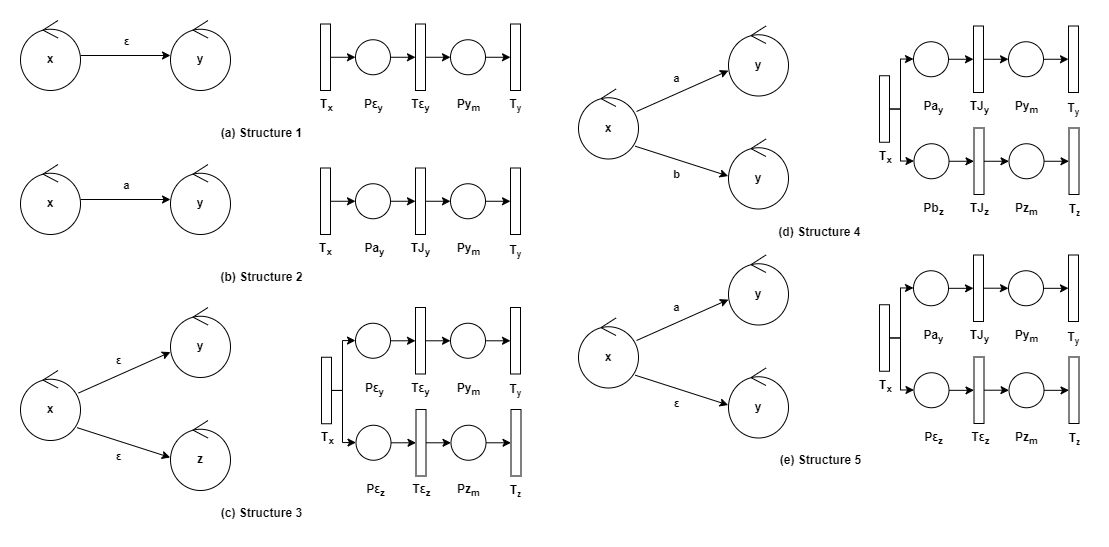
\includegraphics[scale=0.55]{figures/RDLT_TO_PN-Fig1_Yiu et al.png}
            \caption{Structures 1-5 with their equivalent PN \cite{yiu}.}
            \label{s1-5-yiu}
        \end{sidewaysfigure} \par

        \begin{sidewaysfigure}[p]
            \centering
            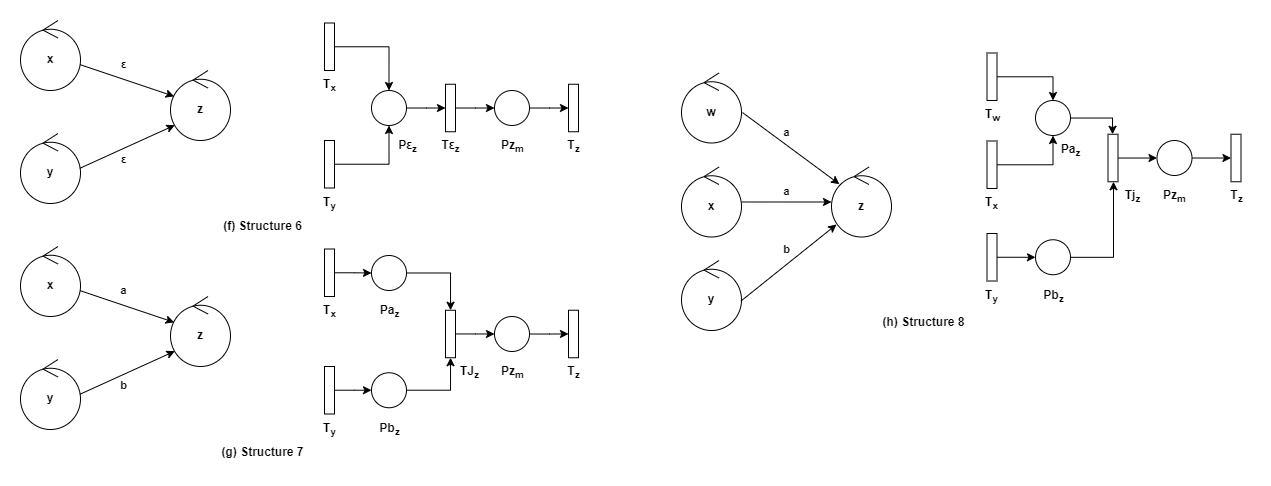
\includegraphics[scale=0.55]{figures/RDLT_TO_PN-Fig2_Yiu et al.png}
            \caption{Structures 6-8 with their equivalent PN \cite{yiu}.}
            \label{s6-8-yiu}
        \end{sidewaysfigure} \par

        \begin{sidewaysfigure}[p]
            \centering
            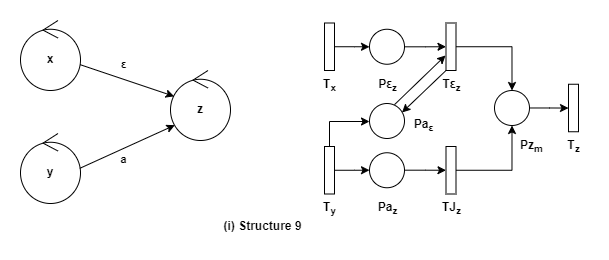
\includegraphics[scale=0.75]{figures/RDLT_TO_PN-Fig3_Yiu et al.png}
            \caption{Structure 9 with equivalent PN \cite{yiu}.}
            \label{s9-yiu}
        \end{sidewaysfigure} \par
        
        Recent literature by Sulla and Malinao \cite{sulla-malinao} builds on the work of Yiu et al. \cite{yiu}, and focuses on developing a novel mapping for the $L$ and $M$-attributes of RDLT to PN. Drawing inspiration from the approach recommended by Yiu et al. \cite{yiu} for mapping $L$-attributes, Sulla and Malinao \cite{sulla-malinao} modified the 9 structures composing an RDLT to support $L$-attributes through the addition of auxiliary places containing a set number of tokens equal to the value of the $L$-attribute of the arc in the RDLT. Each of these auxiliary places is connected to the transitions that represent the traversal of an arc in the RDLT. Then, a reset arc is connected from the auxiliary place to the exit transitions of each structure. Figures \ref{s1-5-sulla-malinao}, \ref{s6-8-sulla-malinao}, and \ref{s9-sulla-malinao} illustrate the 9 RDLT structures and their equivalent modified Petri net which supports the $L$-attribute. Since in some structures, multiple incoming arcs share only one transition, initial token placement rules for auxiliary places in JOIN structures were established. The first rule checks if the $C$-attributes of two incoming arcs from two different vertices are equal, then the number of tokens placed in the auxiliary place is equal to the sum of the $L$-attributes of the two vertices. The second rule, on the other hand, checks whether two incoming arcs from two different vertices are not equal, the vertices are type-alike, and the $C$-attributes of both are $\Sigma$, then the number of tokens placed in the auxiliary place is equal to the least $L$-attribute value between the incoming arcs. Regarding the reset functionality of each structure, if a looping arc is present in the target vertex, a reset arc is not connected to the auxiliary place. Otherwise, a reset arc is connected to the auxiliary place, consuming all tokens once the output transition of the structure is fired. Moreover, all of the auxiliary places created are connected to the transition that is connected to the final output place $o$, which will eventually reset each of these auxiliary places once this transition is fired. This feature is added to ensure that the net will terminate properly, satisfying the condition of classical soundness. As for the mapping of the $M$-attribute, vertex-simplification is performed on the input RDLT with RBS, resulting in two vertex-simplified RDLTs, namely level-1 vertex-simplified RDLT and level-2 vertex-simplified RDLT. The two RDLTs are shown in figure \ref{vertex-simplified-rdlt}. The former is extended by adding a source and a sink place. This describes the overall RDLT with minimized RBS. The latter, on the other hand, describes what is inside the RBS. Then, these two vertex-simplified RDLTs are converted into their equivalent Petri nets. Entering and exiting the RBS is performed through the in-bridges and out-bridges of the RBS itself. With this, the proposed mapping of Sulla and Malinao \cite{sulla-malinao}, checks each vertex if it is an in-bridge or an out-bridge. In the case of an in-bridge, the input place that enables the center of the RBS in level-1 PN is connected to the corresponding transition of that center vertex of RBS in the level-2 PN. For exiting the RBS-equivalent level-2 Petri net, the transition of the source vertex of the out-bridge in the level-2 PN is connected to its corresponding output places in the level-1 PN. The level-1 and level-2 Petri nets are connected by what are essentially XOR splits through the in-bridges and out-bridges. If analysis is to be performed to the level-1 RDLT, then the path through the level-1 PN is followed. Otherwise, if the analysis is to be performed on the internal RBS in the level-2 RDLT, then the path through the level-2 PN is followed instead \cite{sulla-malinao}. This combination of the two Petri Nets, namely level-1 and level-2 PNs, allows simulation and verification of the mapping.

        The presence of MIX-JOINs significantly influences the satisfaction of the soundness property of a given input RDLT. This is a result of how the mapping of that structure was designed to have two transitions sharing a single output place called $P_{zm}$. If both of these transitions fire, then two tokens will be produced in $P_{zm}$, and since by default only one token is consumed by each of the transitions, once a token reaches the final output place $P_{o}$, the output place $P_{zm}$ will still contain one token. This violates the condition of proper termination for classical soundness \cite{sulla-malinao}. The implication of this is that the proposed mapping will result in classical sound PNs if the input RDLT is also classical sound and contains no MIX-JOINs. This is better illustrated in Table \ref{table1} below.

        The algorithm proposed by Sulla and Malinao \cite{sulla-malinao} was proven to have the space complexity of $O(v)$ and time complexity of $O(v^2)$, where v is the number of vertices in the RDLT. Moreover, the mapping is validated by generating an activity profile of the input RDLT and comparing it to its corresponding firing sequence in the output Petri Net. \\

        \begin{table}[h]
            \centering
            \begin{tabular}{|c|c|}
            \hline
            \multicolumn{2}{|c|}{Proposed Mapping Satisfaction of Soundness} \\
            \hline
            Input RDLT & Resulting PN \\
            \hline
            Classical sound RDLT with no MIX-JOIN & Classical Sound \\
            \hline
            Classical sound RDLT with MIX-JOIN & Relaxed Sound \\
            \hline
            Relaxed sound RDLT with no MIX-JOIN & Relaxed Sound \\
            \hline
            Relaxed sound RDLT with MIX-JOIN & Relaxed Sound \\
            \hline
            \end{tabular}
            \caption{Soundness profiles of input RDLT with or without MIX-JOINs and the corresponding soundness profiles of its output Petri Net.}
            \label{table1}
        \end{table}

        \begin{figure}[hb!]
            \centering
            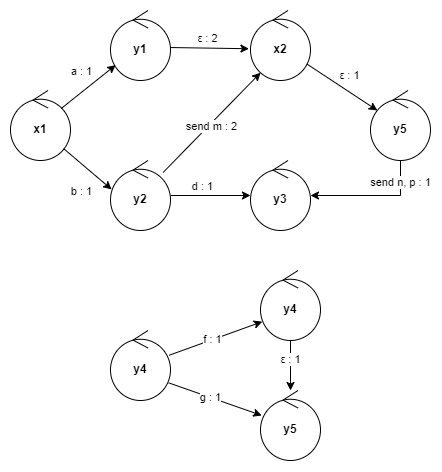
\includegraphics[scale=0.55]{figures/RDLT_TO_PN-Sulla and Malinao_M_Attribute.png}
            \caption{The level-1 and level-2 vertex-simplified RDLT of the RDLT in Figure \ref{rdlt1} \cite{sulla-malinao}.}
            \label{vertex-simplified-rdlt}
        \end{figure} \par

        \begin{sidewaysfigure}[p]
            \centering
            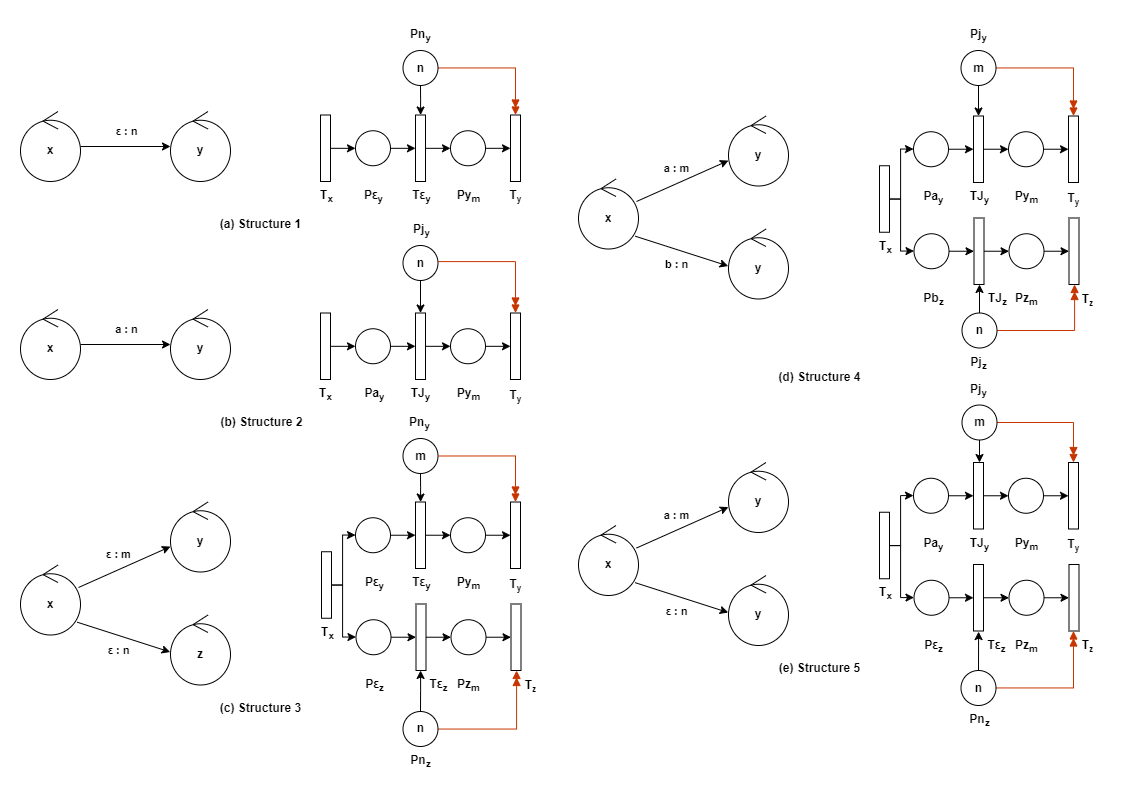
\includegraphics[scale=0.55]{figures/RDLT_TO_PN-Fig1_Sulla and Malinao.png}
            \caption{Modified structures 1-5, that include $L$-attributes with their equivalent PN \cite{sulla-malinao}.}
            \label{s1-5-sulla-malinao}
        \end{sidewaysfigure} \par

        \begin{sidewaysfigure}[p]
            \centering
            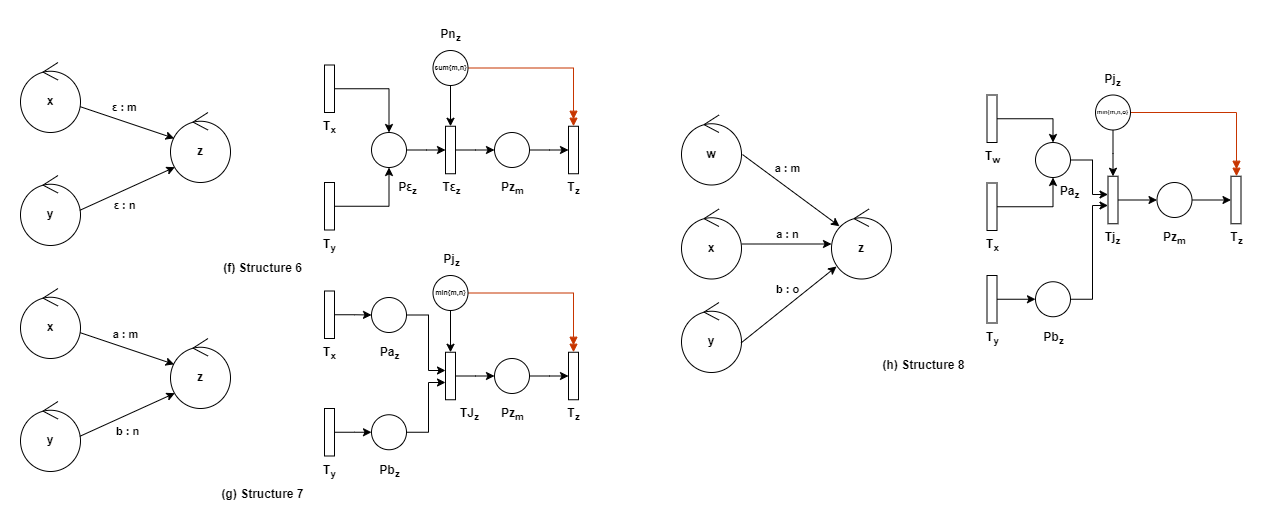
\includegraphics[scale=0.55]{figures/RDLT_TO_PN-Fig2_Sulla and Malinao.png}
            \caption{Modified structures 6-8, that include $L$-attributes with their equivalent PN \cite{sulla-malinao}.}
            \label{s6-8-sulla-malinao}
        \end{sidewaysfigure} \par

        \begin{sidewaysfigure}[p]
            \centering
            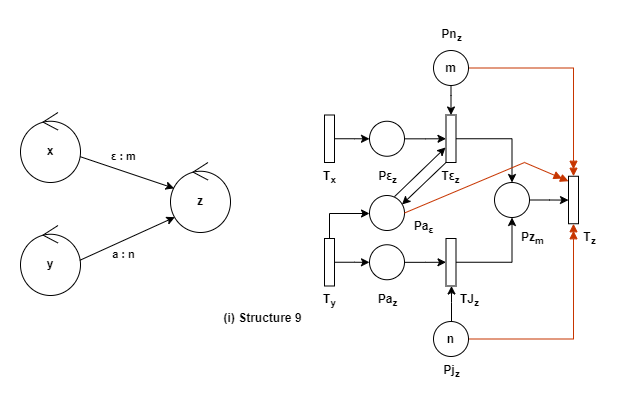
\includegraphics[scale=0.75]{figures/RDLT_TO_PN-Fig3_Sulla and Malinao.png}
            \caption{Modified structure 9, that includes $L$-attributes with their equivalent PN \cite{sulla-malinao}.}
            \label{s9-sulla-malinao}
        \end{sidewaysfigure} \par

        \subsection*{Petri Net Extensions and Variants}
        As stated in the paper of van Der Aalst et al., the basic Petri net model, which is defined in Definition 10, is very plain and straightforward and may sometimes lack the capability to represent elements or components of a complex system one might come across in real life. Fortunately, there are extensions and variants of Petri net that help enhance the expressiveness of the model. Some of these extensions and variants include the use of reset arcs, inhibitor arcs, and arc weights.
        
        A reset arc is represented by an arc with a double-tip arrow attached to one of its edges \cite{sulla-malinao}. Unlike the regular arc, this component does not impact the enabling of transitions. However, once a transition connected to a reset arc is fired, all the tokens inside the input place connected by a reset arc are removed. Inhibitor arcs are counter-intuitive to a normal arc in the sense that they prevent a transition from firing when there is at least one (1) token in its input place.  Albeit different from a reset arc, it was shown to emulate the behavior of reset arcs \cite{vanderaals-soundness-wfn}. Inhibitor arcs are represented by an arc with a small circle, instead of an arrow, at the edge where it is connected to the transition \cite{pertsukhov-mitsyuk}. The weight of an arc represents the number of tokens required and produced by the input and output arc of a transition, respectively. This means that the weight of an input arc of a transition represents the number of tokens that will be consumed by the transition, and the weight of an output arc of a transition shows the number of tokens that the transition will produce to its output place. A study by Pertsukhov and Mitsyuk \cite{pertsukhov-mitsyuk} presented an approach and a tool for simulating Petri nets with reset arcs, inhibitor arcs, and arc weights. In their paper, process model simulation was applied to successfully generate event logs. They defined event logs as a finite multi-set of traces, where a trace is a finite sequence of events \cite{pertsukhov-mitsyuk}. A separate study by van der Aalst et al. \cite{vanderaalst-etal} explored the decidability of soundness notions in the presence of cancellation using a workflow model called RWF net or Reset Workflow net. The RWF net is a reset net that has additional components, such as source and sink places. It also ensures that every node in the net is a path from the source place to the sink place and that there is no reset arc connected to the sink place \cite{vanderaalst-etal}. The authors were able to show that the classical notion of soundness becomes undecidable by adding reset arcs to the net. This also applies to the less strict notion of soundness, the relaxed soundness. Moreover, it was observed that soundness can be verified for RWF-nets with a finite state space, and even if the state space is infinitely large, a partial exploration of the space may reveal different errors.

        The results and findings of the different literature will give insight into what Petri net components, variants, and extensions will be used in this paper. Furthermore, the different notions of soundness will also help to ensure the reliability and correctness of the proposed mapping.
        % \subsection*{Soundness in Petri nets}